\begin{figure}[H]
\centering
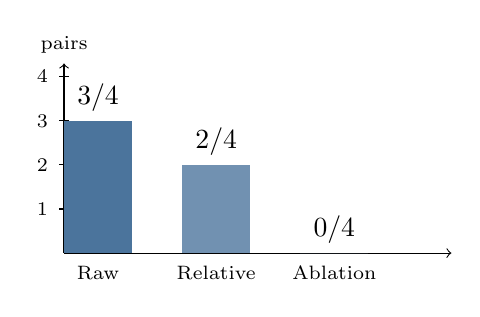
\begin{tikzpicture}[x=1.2cm,y=0.56cm]
\definecolor{diagblue}{RGB}{43,91,139}
\draw[->] (0,0) -- (4.1,0);
\draw[->] (0,0) -- (0,4.3) node[above,font=\scriptsize] {pairs};
\foreach \y in {1,2,3,4} {\draw (-0.05,\y) -- (0.05,\y) node[left,xshift=-4pt,font=\scriptsize] {\y};}
\fill[diagblue!85] (0.00,0) rectangle (0.72,3);
\node[above] at (0.36,3) {3/4};
\node[below,align=center,font=\scriptsize] at (0.36,-0.08) {Raw};
\fill[diagblue!67] (1.25,0) rectangle (1.97,2);
\node[above] at (1.61,2) {2/4};
\node[below,align=center,font=\scriptsize] at (1.61,-0.08) {Relative};
\fill[diagblue!49] (2.50,0) rectangle (3.22,0);
\node[above] at (2.86,0) {0/4};
\node[below,align=center,font=\scriptsize] at (2.86,-0.08) {Ablation};
\end{tikzpicture}
\caption{Paired mechanism discrimination in four frozen Incident 003 v3 development constructions. Raw counts only; no uncertainty bars or equivalence claim.}
\label{fig:paired}
\end{figure}
